
%(BEGIN_QUESTION)
% Copyright 2012, Tony R. Kuphaldt, released under the Creative Commons Attribution License (v 1.0)
% This means you may do almost anything with this work of mine, so long as you give me proper credit

This control system controls ``waste'' fuel gas header pressure by venting gas into the burner.  It also limits the flow of ``waste'' gas when excessive, through the use of an override control strategy.  The blue-colored, italicized numbers indicate ``live'' signal values at one point in time:

$$\includegraphics[width=15.5cm]{i01151x01.eps}$$

Determine the following signal value percentages based on the given values and the expected behavior of the control system, assuming each of the selected controllers is operating with PV precisely equal to SP:

\begin{itemize}
\item{} Process variable of controller FC-5 = \underbar{\hskip 50pt}
\vskip 10pt
\item{} Output of controller FC-5 = \underbar{\hskip 50pt}
\vskip 10pt
\item{} Process variable of controller FC-8 = \underbar{\hskip 50pt}
\vskip 10pt
\item{} Setpoint of controller FC-8 = \underbar{\hskip 50pt}
\end{itemize}

\underbar{file i01151}
%(END_QUESTION)





%(BEGIN_ANSWER)

{\it 3 points for each of the first three answers; 1 point for the setpoint of FC-8}:

\begin{itemize}
\item{} Process variable of controller FC-5 = \underbar{\bf 48\%}
\item{} Output of controller FC-5 = \underbar{\bf 31\%}
\item{} Process variable of controller FC-8 = \underbar{\bf 12\%}
\item{} Setpoint of controller FC-8 = \underbar{\bf 12\%}
\end{itemize}

%(END_ANSWER)





%(BEGIN_NOTES)

{\bf This question is intended for exams only and not worksheets!}.

%(END_NOTES)


